\chapter{The Real Number System ($\mathbb{R}$)}
\label{chap:real_numbers}

\section{Axiomatic Structure of the Real Field}

The set of real numbers $\mathbb{R}$ is axiomatically characterized as a **complete, Archimedean, totally ordered field**. While the rational numbers $\mathbb{Q}$ form an ordered field, they exhibit fatal topological "gaps" (such as $\sqrt{2} \notin \mathbb{Q}$ or $\pi \notin \mathbb{Q}$). The construction of $\mathbb{R}$ seals every gap through the **Completeness Axiom**.

\begin{figure}[htbp]
  \centering
  \begin{minipage}{0.35\textwidth}
    \centering
    
\includegraphics[width=0.82\textwidth]{cantor.jpg}
    \caption*{(a) \textbf{Georg Cantor (1845--1918)}}
  \end{minipage}
  \hspace{0.08\textwidth}
  \begin{minipage}{0.35\textwidth}
    \centering
    
\includegraphics[width=0.82\textwidth]{dedekind.jpg}
    \caption*{(b) \textbf{Richard Dedekind (1831--1916)}}
  \end{minipage}
  \caption{\textbf{Founders of Real Analysis:} Georg Cantor (inventor of transfinite set theory and diagonal cardinality) and Richard Dedekind (creator of Dedekind cuts, providing the first rigorous construction of the real continuum $\mathbb{R}$ from $\mathbb{Q}$).}
  \label{fig:cantor_dedekind}
\end{figure}

\begin{definitionbox}{Absolute Value and Distance on $\mathbb{R}$}
For any real number $x \in \mathbb{R}$, its \textbf{absolute value} $|x|$ is defined by:
\[
|x| = \begin{cases} x & \text{if } x \ge 0, \\ -x & \text{if } x < 0. \end{cases} \iff |x| = \max(x, -x) = \sqrt{x^2}.
\]
The Euclidean distance between two numbers $x, y \in \mathbb{R}$ is $d(x, y) = |x - y|$.
\end{definitionbox}

\begin{theorembox}{The Triangle Inequalities}
For all real numbers $x, y \in \mathbb{R}$:
\begin{enumerate}[leftmargin=1.4em,itemsep=3pt]
  \item \textbf{Standard Triangle Inequality:}
  \[
  |x + y| \le |x| + |y|.
  \]
  Equality holds if and only if $x$ and $y$ have the same sign ($x y \ge 0$).
  \item \textbf{Reverse Triangle Inequality:}
  \[
  \big| |x| - |y| \big| \le |x - y|.
  \]
  \item \textbf{Generalized $n$-term Inequality:}
  \[
  \left| \sum_{k=1}^n x_k \right| \le \sum_{k=1}^n |x_k|.
  \]
\end{enumerate}
\end{theorembox}

\section{Bounded Sets, Maximum, Minimum, Supremum and Infimum}

\begin{definitionbox}{Upper Bounds, Lower Bounds, Extrema}
Let $A$ be a non-empty subset of $\mathbb{R}$ ($A \subseteq \mathbb{R}, A \neq \emptyset$):
\begin{enumerate}[leftmargin=1.4em,itemsep=3pt]
  \item \textbf{Bounded Above (Majoré):} $\exists M \in \mathbb{R}, \ \forall x \in A, \ x \le M$. $M$ is an \textbf{upper bound} (majorant).
  \item \textbf{Bounded Below (Minoré):} $\exists m \in \mathbb{R}, \ \forall x \in A, \ x \ge m$. $m$ is a \textbf{lower bound} (minorant).
  \item \textbf{Bounded Set (Borné):} $A$ is both bounded above and below:
  \[
  \exists K > 0, \quad \forall x \in A, \quad |x| \le K.
  \]
  \item \textbf{Maximum (Greatest Element):} An upper bound $M$ that \textbf{belongs to the set}:
  \[
  M = \max A \iff (M \in A \ \land \ \forall x \in A, x \le M).
  \]
  \item \textbf{Minimum (Least Element):} A lower bound $m$ that belongs to the set:
  \[
  m = \min A \iff (m \in A \ \land \ \forall x \in A, x \ge m).
  \]
\end{enumerate}
\end{definitionbox}

\begin{figure}[htbp]
  \centering
  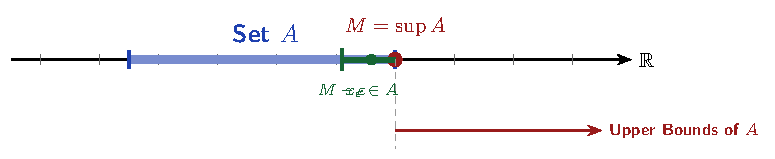
\includegraphics[width=0.88\textwidth]{03_real_completeness.pdf}
  \caption{\textbf{The Completeness Axiom and Supremum Characterization:} The supremum $M = \sup A$ is the least upper bound. For any arbitrary small $\varepsilon > 0$, the interval $(M - \varepsilon, M]$ contains at least one element $x_\varepsilon \in A$.}
  \label{fig:completeness}
\end{figure}

\begin{theorembox}{The Axiom of Completeness (Axiom of the Supremum)}
Every non-empty subset $A \subset \mathbb{R}$ that is bounded above possesses a \textbf{least upper bound} in $\mathbb{R}$, denoted $\sup A$ (\textbf{supremum} or \textit{borne supérieure}).

Similarly, every non-empty subset $A \subset \mathbb{R}$ that is bounded below possesses a \textbf{greatest lower bound} in $\mathbb{R}$, denoted $\inf A$ (\textbf{infimum} or \textit{borne inférieure}).
\end{theorembox}

\begin{propbox}{Analytical $\varepsilon$-Characterization of Supremum and Infimum}
Let $A \subset \mathbb{R}$ be non-empty and bounded above. A real number $S \in \mathbb{R}$ is the supremum ($S = \sup A$) if and only if:
\begin{equation}
\begin{cases}
(1) & \forall x \in A, \quad x \le S \quad (\text{$S$ is an upper bound}) \\
(2) & \forall \varepsilon > 0, \quad \exists x_\varepsilon \in A \ \text{such that} \ x_\varepsilon > S - \varepsilon \quad (\text{no smaller upper bound exists})
\end{cases}
\end{equation}
Similarly, $I = \inf A$ if and only if:
\begin{equation}
\begin{cases}
(1) & \forall x \in A, \quad x \ge I \quad (\text{$I$ is a lower bound}) \\
(2) & \forall \varepsilon > 0, \quad \exists x_\varepsilon \in A \ \text{such that} \ x_\varepsilon < I + \varepsilon
\end{cases}
\end{equation}
\end{propbox}

\section{The Archimedean Property and Density}

\begin{theorembox}{The Archimedean Property of $\mathbb{R}$}
The real number field $\mathbb{R}$ is \textbf{Archimedean}: it contains no infinitely large or infinitesimally small elements.
\begin{equation}
\forall x \in \mathbb{R}, \quad \exists n \in \mathbb{N} \quad \text{such that} \quad n > x.
\end{equation}
\textbf{Fundamental Analytical Equivalences:}
\begin{enumerate}[leftmargin=1.4em,itemsep=2pt]
  \item $\forall \varepsilon > 0, \ \exists n \in \mathbb{N}^* \ \text{such that} \ \frac{1}{n} < \varepsilon$.
  \item $\forall x, y \in \mathbb{R}$ with $x > 0$, $\exists n \in \mathbb{N}$ such that $n x > y$.
  \item The set of natural numbers $\mathbb{N}$ is not bounded above in $\mathbb{R}$ ($\sup \mathbb{N} = +\infty$).
\end{enumerate}
\end{theorembox}

\begin{propbox}{The Floor Function (Integer Part)}
For every real number $x \in \mathbb{R}$, there exists a **unique** integer $p \in \mathbb{Z}$ such that:
\begin{equation}
p \le x < p + 1.
\end{equation}
This integer is the \textbf{integer part} (or floor) of $x$, denoted $E(x) \equiv \lfloor x \rfloor = p$.
\end{propbox}

\begin{theorembox}{Density of Rational and Irrational Numbers in $\mathbb{R}$}
Between any two distinct real numbers, there exist infinitely many rational numbers and infinitely many irrational numbers:
\begin{equation}
\forall a, b \in \mathbb{R} \ \text{with} \ a < b, \quad \exists r \in \mathbb{Q} \ \text{and} \ \exists \alpha \in \mathbb{R} \setminus \mathbb{Q} \quad \text{such that} \quad a < r < \alpha < b.
\end{equation}
In topological terms, both $\mathbb{Q}$ and $\mathbb{R} \setminus \mathbb{Q}$ are \textbf{dense} in $\mathbb{R}$ ($\overline{\mathbb{Q}} = \mathbb{R}$ and $\overline{\mathbb{R} \setminus \mathbb{Q}} = \mathbb{R}$).
\end{theorembox}

\section{Worked Examples with Step-by-Step Proofs}

\begin{workedexample}{Rigorous Proof of the Archimedean Property from Completeness}
Prove rigorously that the Archimedean property ($\forall x \in \mathbb{R}, \exists n \in \mathbb{N}: n > x$) is a direct consequence of the Completeness Axiom of $\mathbb{R}$.

\paragraph{Solution and Proof.}
We proceed by contradiction (\textit{reductio ad absurdum}).
Assume that the Archimedean property is false. Then its logical negation is true:
\[
\exists x_0 \in \mathbb{R}, \quad \forall n \in \mathbb{N}, \quad n \le x_0.
\]
This statement asserts that $x_0$ is an \textbf{upper bound} for the set of natural numbers $\mathbb{N} \subset \mathbb{R}$.
Therefore, $\mathbb{N}$ is a non-empty subset of $\mathbb{R}$ bounded above by $x_0$.

By the \textbf{Completeness Axiom}, $\mathbb{N}$ must possess a supremum in $\mathbb{R}$:
\[
S = \sup \mathbb{N} \in \mathbb{R}.
\]
Now consider $\varepsilon = 1 > 0$.
By the $\varepsilon$-characterization of the supremum, $S - 1$ is strictly strictly smaller than $S$, so $S - 1$ \textbf{cannot be an upper bound} of $\mathbb{N}$.
Therefore, there exists at least one element $m \in \mathbb{N}$ such that:
\[
m > S - 1.
\]
Adding $1$ to both sides of this inequality:
\[
m + 1 > S.
\]
Since $m \in \mathbb{N}$, its successor $m + 1$ is also a natural number ($m + 1 \in \mathbb{N}$).
Thus, we have found an element of $\mathbb{N}$ that is strictly strictly greater than $S = \sup \mathbb{N}$.
This contradicts the fundamental definition of $S$ as an upper bound of $\mathbb{N}$!

Therefore, the assumption is impossible, establishing that:
\[
\mathbf{\forall x \in \mathbb{R}, \quad \exists n \in \mathbb{N} \quad \text{such that} \quad n > x}. \quad \blacksquare
\]
\end{workedexample}

\begin{workedexample}{Determining $\sup, \inf, \max, \min$ of a Real Set}
Consider the set:
\[
A = \left\{ \frac{2n - 1}{n + 2} \;\middle|\; n \in \mathbb{N}^* \right\} = \left\{ \frac{1}{3}, \frac{3}{4}, \frac{5}{5}, \frac{7}{6}, \dots \right\}.
\]
\begin{enumerate}[leftmargin=1.4em,itemsep=2pt]
  \item Determine $\min A$ and $\inf A$, proving your answer rigorously.
  \item Prove that $A$ has no maximum ($\max A$ does not exist).
  \item Determine $\sup A$ using the $\varepsilon$-characterization property.
\end{enumerate}

\paragraph{Solution and Proof.}
Rewrite the general element $x_n = \frac{2n - 1}{n + 2}$ by polynomial division:
\[
x_n = \frac{2(n + 2) - 5}{n + 2} = 2 - \frac{5}{n + 2}.
\]
\textbf{1. Infimum and Minimum:}
As $n$ increases ($n \in \{1, 2, 3, \dots\}$), the denominator $n+2$ increases, so $\frac{5}{n+2}$ strictly decreases.
Therefore, $x_n = 2 - \frac{5}{n+2}$ is a \textbf{strictly increasing sequence}:
\[
x_1 = 2 - \frac{5}{3} = \frac{1}{3}, \quad x_2 = 2 - \frac{5}{4} = \frac{3}{4}, \quad \dots
\]
For all $n \ge 1$:
\[
x_n \ge x_1 = \frac{1}{3}.
\]
Thus $1/3$ is a lower bound of $A$. Moreover, since $1/3 = x_1 \in A$:
\[
\mathbf{\min A = \inf A = \frac{1}{3}}.
\]

\textbf{2. Non-existence of Maximum:}
Since $n+2 > 0$ for all $n \ge 1$, $\frac{5}{n+2} > 0$, which means:
\[
x_n = 2 - \frac{5}{n+2} < 2 \quad \text{for all } n \in \mathbb{N}^*.
\]
Thus $2$ is an upper bound of $A$, but $2 \notin A$ (since $2 - \frac{5}{n+2} = 2 \implies \frac{5}{n+2} = 0$, which has no real solution).
Because the sequence $x_n$ is strictly increasing, every element $x_n$ is strictly smaller than $x_{n+1} \in A$.
Therefore, no single element in $A$ can be the greatest element: $\mathbf{\max A \text{ does not exist}}$.

\textbf{3. Supremum Determination via $\varepsilon$-Characterization:}
We claim that $\sup A = 2$.
\begin{itemize}[leftmargin=1.4em,itemsep=2pt]
  \item \textbf{Condition 1 (Upper Bound):} We already showed $\forall n \ge 1, x_n < 2$. Thus $2$ is an upper bound.
  \item \textbf{Condition 2 ($\varepsilon$-Condition):} Let $\varepsilon > 0$ be given. We must find an integer $n \in \mathbb{N}^*$ such that:
  \[
  x_n > 2 - \varepsilon \iff 2 - \frac{5}{n + 2} > 2 - \varepsilon \iff \frac{5}{n + 2} < \varepsilon \iff n + 2 > \frac{5}{\varepsilon} \iff n > \frac{5}{\varepsilon} - 2.
  \]
  By the Archimedean property of $\mathbb{R}$, there always exists an integer $n_0 \in \mathbb{N}^*$ such that $n_0 > \frac{5}{\varepsilon} - 2$.
  Choosing this $n_0$, we have $x_{n_0} \in A$ and $x_{n_0} > 2 - \varepsilon$.
\end{itemize}
Both conditions of the $\varepsilon$-characterization are satisfied. Therefore:
\[
\mathbf{\sup A = 2}. \quad \blacksquare
\]
\end{workedexample}

\begin{workedexample}{Density Proof: Constructing a Rational Between Any Two Reals}
Prove rigorously that for any real numbers $x, y \in \mathbb{R}$ with $x < y$, there exists a rational number $r \in \mathbb{Q}$ such that:
\[
x < r < y.
\]

\paragraph{Solution and Proof.}
Since $x < y$, the interval length is strictly positive: $y - x > 0$.
\begin{enumerate}[leftmargin=1.4em,itemsep=3pt]
  \item \textbf{Choice of Denominator $n$:}
  By the Archimedean property, there exists an integer $n \in \mathbb{N}^*$ such that:
  \[
  n > \frac{1}{y - x} \iff \frac{1}{n} < y - x \iff n y - n x > 1.
  \]
  \item \textbf{Choice of Numerator $m$:}
  Consider the number $n x$. By the floor function property, there exists a unique integer $m \in \mathbb{Z}$ such that:
  \[
  m - 1 \le n x < m \iff n x < m \le n x + 1.
  \]
  \item \textbf{Verification of Inequalities:}
  From the left inequality:
  \[
  n x < m \implies x < \frac{m}{n}.
  \]
  From the right inequality and since $n y - n x > 1 \implies n x + 1 < n y$:
  \[
  m \le n x + 1 < n y \implies m < n y \implies \frac{m}{n} < y.
  \]
  Combining both inequalities:
  \[
  x < \frac{m}{n} < y.
  \]
\end{enumerate}
Setting $r = \frac{m}{n} \in \mathbb{Q}$, we have established that $\mathbf{x < r < y}$. $\blacksquare$
\end{workedexample}

\begin{workedexample}{Supremum of a Two-Variable Bounded Set}
Let $A$ and $B$ be two non-empty subsets of $\mathbb{R}$ bounded above. Define:
\[
A + B = \{ x + y \mid x \in A \land y \in B \}.
\]
Prove that $A + B$ is bounded above and that:
\[
\sup(A + B) = \sup A + \sup B.
\]

\paragraph{Solution and Proof.}
Let $S_A = \sup A$ and $S_B = \sup B$.
\begin{enumerate}[leftmargin=1.4em,itemsep=3pt]
  \item \textbf{$S_A + S_B$ is an Upper Bound for $A + B$:}
  Let $z \in A + B$. By definition, $z = x + y$ with $x \in A$ and $y \in B$.
  Since $S_A$ is an upper bound of $A$, $x \le S_A$.
  Since $S_B$ is an upper bound of $B$, $y \le S_B$.
  Adding the two inequalities:
  \[
  z = x + y \le S_A + S_B.
  \]
  Since this holds for every $z \in A + B$, $A + B$ is bounded above by $S_A + S_B$.
  By the Completeness Axiom, $\sup(A + B)$ exists, and:
  \[
  \sup(A + B) \le S_A + S_B.
  \]

  \item \textbf{Reverse Inequality via $\varepsilon$-Characterization:}
  Let $\varepsilon > 0$ be given. Consider $\varepsilon' = \frac{\varepsilon}{2} > 0$.
  \begin{itemize}[leftmargin=1.4em,itemsep=2pt]
    \item By the $\varepsilon$-characterization of $\sup A$, there exists $x_0 \in A$ such that $x_0 > S_A - \frac{\varepsilon}{2}$.
    \item By the $\varepsilon$-characterization of $\sup B$, there exists $y_0 \in B$ such that $y_0 > S_B - \frac{\varepsilon}{2}$.
  \end{itemize}
  Adding these two inequalities:
  \[
  x_0 + y_0 > \left( S_A - \frac{\varepsilon}{2} \right) + \left( S_B - \frac{\varepsilon}{2} \right) = (S_A + S_B) - \varepsilon.
  \]
  Since $x_0 + y_0 \in A + B$, we have found an element of $A + B$ strictly greater than $(S_A + S_B) - \varepsilon$.
  Therefore, no number strictly smaller than $S_A + S_B$ can be an upper bound for $A + B$.
  This proves that:
  \[
  \sup(A + B) \ge S_A + S_B.
  \]
\end{enumerate}
Combining both inequalities yields the exact equality:
\[
\mathbf{\sup(A + B) = \sup A + \sup B}. \quad \blacksquare
\]
\end{workedexample}
